\section{Method}
\label{sec:method}
%The synergy between ontologies and data mining can be achieved by employing the RDF model given the fact that RDF allows a combined specification of both schema information and data structured under the schema. In light of Hayes et al.'s proposal to represent RDF as hypergraphs~\cite{GraphModelRDF}, we develop a set of rules to represent data in transactional tables as hypergraphs or bipartite graphs with minimal loss of semantics. We then propose a novel way to combine the graph representations of data and domain knowledge encoded in ontologies as a unified information source from which valuable insights can be drawn upon.

\subsection{Graph Representation for Biomedical Ontologies}
The Web Ontology Language (OWL~\cite{OWL}) is the W3C's standard for representing Semantic Web ontologies and has been adopted by most biomedical ontology development efforts. OWL ontologies can be used along with RDF data because OWL uses the RDF syntax. RDF's abstract triple syntax has a graph nature. The RDF graph is defined as a set of triples and can be viewed as a \emph{directed labeled graph} (DG):

\hspace{.6in}\ovalbox{subject} $\stackbin[]{predicate}{\xrightarrow{\hspace*{2cm}}}$ \ovalbox{object}\;.

One disadvantage of DG is that it makes an artificial distinction between resources and properties, which leads to incongruous representations. Consider the RDF statements in the following example:

$\langle$\textit{Lipitor has\_ingredient Active\_Ingredient}$\rangle$, \\
$\langle$\textit{Active\_Ingredient has\_chemical Atorvastatin\_Calcium}$\rangle$,\\
$\langle$\textit{has\_chemical subPropertyOf has\_ingredient}$\rangle$. 

From the first two statements, \textit{Lipitor} (a drug made by Pfizer), \textit{Active\_Ingredient} and \textit{Atorvastatin\_Calcium} can be represented in a DG as nodes connected by edges \textit{has\_ingredient} and \textit{\textit{has\_chemical}} respectively. However, from the last statement, to express the relationship between \textit{has\_chemical} and \textit{has\_ingredient}, these concepts have to be represented as nodes themselves. Representing this set of statements in DG inevitably separates the information into two inconsistent subgraphs, making it difficult for graph-based methods to utilize the information in a holistic and systematic manner.

%Haishan, please change to a biomedical example?  For example, drug X may_treat Disease Y, etc ...


To overcome the inconsistency, Hayes et al.~\cite{GraphModelRDF} proposed to model RDF as a \emph{hypergraph}. A hypergraph~\cite{Hypergraph} is a generalization of a traditional graph where edges, called hyperedges, can connect more than two vertices. If each edge in a hypergraph covers the same number of nodes, it is called $r$-uniform hypergraph, $r$ being the number of nodes on each edge. Any RDF graph can be represented by a simple ordered 3-uniform hypergraph, in which an RDF triple corresponds to a hyperedge, with incident nodes being the subject, predicate and object from the triple. In this way, both meta-data and data level statements can be integrated in a consistent graph representation.

Formally, a hypergraph $HG = (V,E)$, is a pair in which $V$ is the vertex set and $E$ is the hyperedge set where each $e \in E$ is a subset of $V$. A weighted hypergraph is a hypergraph that has a positive number $w(e)$ associated with each hyperedge; called the weight of hyperedge. A weighted hypergraph can be denoted by $G = (V,E,W)$. Furthermore, A hypergraph $HG = (V, E)$ can be transformed to an \emph{bipartite graph} $BG$ as follows: let the node sets $V$ and $E$ be the two parts of $BG$. Then $(v_1, e_1)$ is connected with an edge if and only if vertex $v_1$ is contained in the hyperedge $e_1$ of $HG$. In other words, the incidence matrix of $HG$ can be viewed as the node adjacency (biadjacency) matrix of the bipartite graph.

BG have many desirable properties for developing intuitive mining algorithms because they turn hypergraphs into a simple form so that many algorithms designed on simple graphs can be readily applied. Therefore, we propose to use bipartite graphs to represent domain knowledge and data expressed in RDF.

\subsection{Graph representation for Ontology-Anno\-tated Data}
There already exist methods for transforming data, such as those in relation databases, into RDF~\cite{RDB2RDF}. An ontology-annotation, as we see it, is a binary value representing whether some ontological concept (or class) is associated with some entity.  Often, this means that some concept appears in some document and thus the ontology serves to index the document with related concepts~\cite{RI}.  Thus, we can think of ontology-annotations as a table, with each row representing an entity (e.g., a document), and each column is a class from some ontology.  Cells having a ``1'' denotes that the document \emph{mentions} the term defined by the class.  RDF can be seen as a sparse matrix representation of this data (Table~\ref{tbl:binary-rel}).  This idea can be easily extended to nominal-valued tables as well, or with other relationships besides \emph{mentions} as we illustrate when discussing unified bipartite graphs in the next section.
\begin{table}[ht]
\begin{minipage}[b]{0.38\linewidth}\begin{flushright}
\begin{tabular}{ c | c | c | c |}
\cline{2-4}
	~   & $f_1$	    & $\cdots$  & $f_n$   \\
\cline{2-4}
$r_1:$	&  0  	& $\cdots$   &    1  \\
\cline{2-4}
$\vdots$& $\vdots$  & $\ddots$  & $\vdots$\\
\cline{2-4}
$r_m:$	&  1  	& $\cdots$   &    0  \\
\cline{2-4}
\end{tabular}
\end{flushright}
\end{minipage}
\hfill
\begin{minipage}[b]{0.4\linewidth}
\begin{tabular}{c c c}
\emph{s}&   \emph{p}&  \emph{o}\\
\texttt{<$r_1$}   &    \texttt{mentions}   &  \texttt{$f_n$>}\\
\texttt{<$r_m$}   &    \texttt{mentions}   &  \texttt{$f_1$>}\\
\end{tabular}
\end{minipage}
\begin{minipage}[c]{0.4\linewidth}\centering
\vspace{0.2cm}\hspace{1.5cm}(A)
\end{minipage}
\begin{minipage}[c]{0.4\linewidth}\centering
\hspace{2.6cm}(B)
\end{minipage}
\caption{\label{tbl:binary-rel} Ontology-annotated data (A) is a feature matrix attributing classes from ontologies, $f_i$, to entities such as documents, $r_j$, that is easily represented in sparse matrix form using RDF triples (B).}
\end{table}

\subsection{Unified Graph Representation for Biomedical Ontologies and Data}
In order to facilitate the synergy between data and domain knowledge, information from both sources needs to be first combined. This is achieved by the process called \emph{semantic annotation}. Semantic annotation aims at assigning formal semantic descriptions to the basic element of data, and it is crucial in realizing semantic data mining by bridging formal semantics in domain knowledge with data. If data is annotated, a unified graph incorporating information from both data and ontologies can be created. The following example demonstrates the combination of an ontology graph and a data graph.

Figure~\ref{fig:onto-and-data} (A) shows a simple ontology with only subsumption relationships defined for five entities (A--E) representing, for example, concepts in the biomedical domain. Figure~\ref{fig:onto-and-data} (B) is a binary-valued RDB table in the same domain A--E being column headers (features). We use the same concept labels in the ontology and the RDB table because we assume the mapping between the ontology nodes and the table features are pre-assigned manually or established by automatic annotation. Figure~\ref{fig:hypergraph-combined} (B) shows the RDF statements derived from both the ontology and the RDB table. Figure~\ref{fig:hypergraph-combined} (A) demonstrates the unified RDF bipartite graph.

%Again, can we give medical terms for A, B, C, D, E, you don't need to re-draw the figure, you just need to say five concepts, A is �, B is �.


\begin{figure*}[tbh]
\begin{minipage}[c]{.4\textwidth}\centering
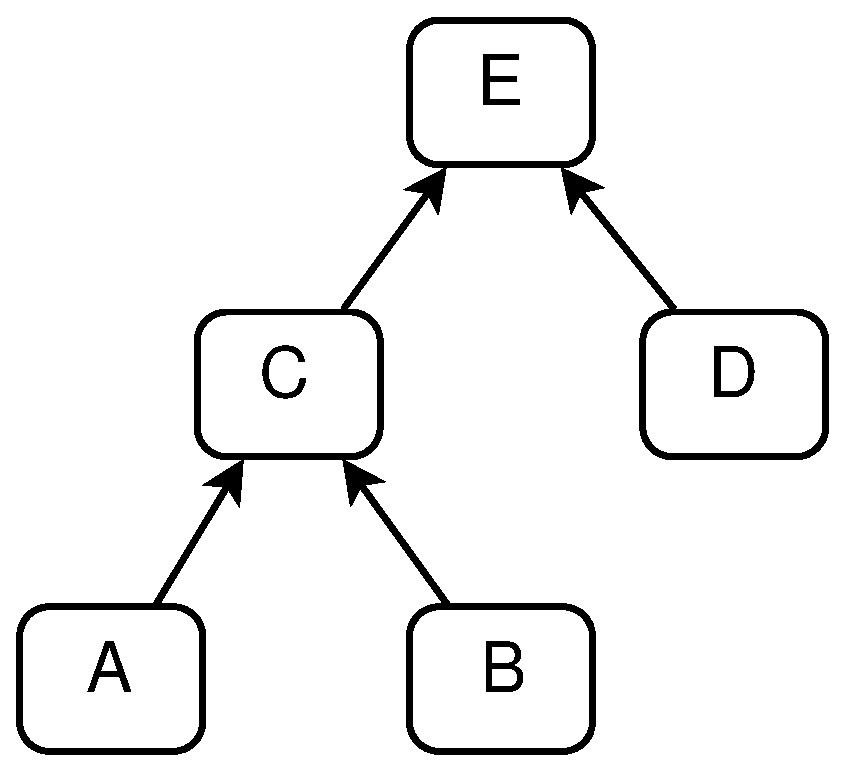
\includegraphics[width=.45\linewidth]{fig/simple-onto.eps}
\end{minipage}
\begin{minipage}[c]{.25\textwidth}\centering
    \begin{tabular}{ c | c | c | c | c | c |}
    \cline{2-6}
    	~ & A & B & C & D & E\\
    \cline{2-6}
    $A:$& 0 & 0 & 1 & 0 & 0 \\
    \cline{2-6}
    $B:$& 0 & 0 & 1 & 0 & 0 \\
    \cline{2-6}
    $C:$& 0 & 0 & 0 & 0 & 1 \\
    \cline{2-6}
    $D:$& 0 & 0 & 0 & 0 & 1 \\
    \cline{2-6}
    $E:$& 0 & 0 & 0 & 0 & 0 \\
    \cline{2-6}
    \end{tabular}
\end{minipage}
\begin{minipage}[c]{.25\textwidth}\centering
    \begin{tabular}{ c | c | c | c | c | c |}
    \cline{2-6}
    	~ & A & B & C & D & E\\
    \cline{2-6}
    $r_1:$& 1 & 1 & 0 & 0 & 0 \\
    \cline{2-6}
    $r_2:$& 1 & 1 & 1 & 0 & 0 \\
    \cline{2-6}
    $r_3:$& 0 & 1 & 1 & 0 & 0 \\
    \cline{2-6}
    $r_3:$& 0 & 0 & 0 & 1 & 0 \\
    \cline{2-6}
    \end{tabular}
\end{minipage}
\begin{minipage}[c]{0.4\linewidth}\centering
(A)
\end{minipage}
\begin{minipage}[c]{0.25\linewidth}\centering
(B)
\end{minipage}
\begin{minipage}[c]{0.25\linewidth}\centering
(C)
\end{minipage}
\caption{\label{fig:onto-and-data} Five concepts (\emph{A--E}) are represented visually as a hierarchy (A) and also as a a hypergraph using the binary feature matrix (B), where a ``1'' denotes \emph{rdfs:subClassOf}, which is similar to the ontology-annotated data (C), where ``1'' denotes \emph{mentions}.}
\end{figure*}

\begin{figure*}[tbh]
\begin{center}
\begin{tabular}{c  c}
\multirow{12}{*}{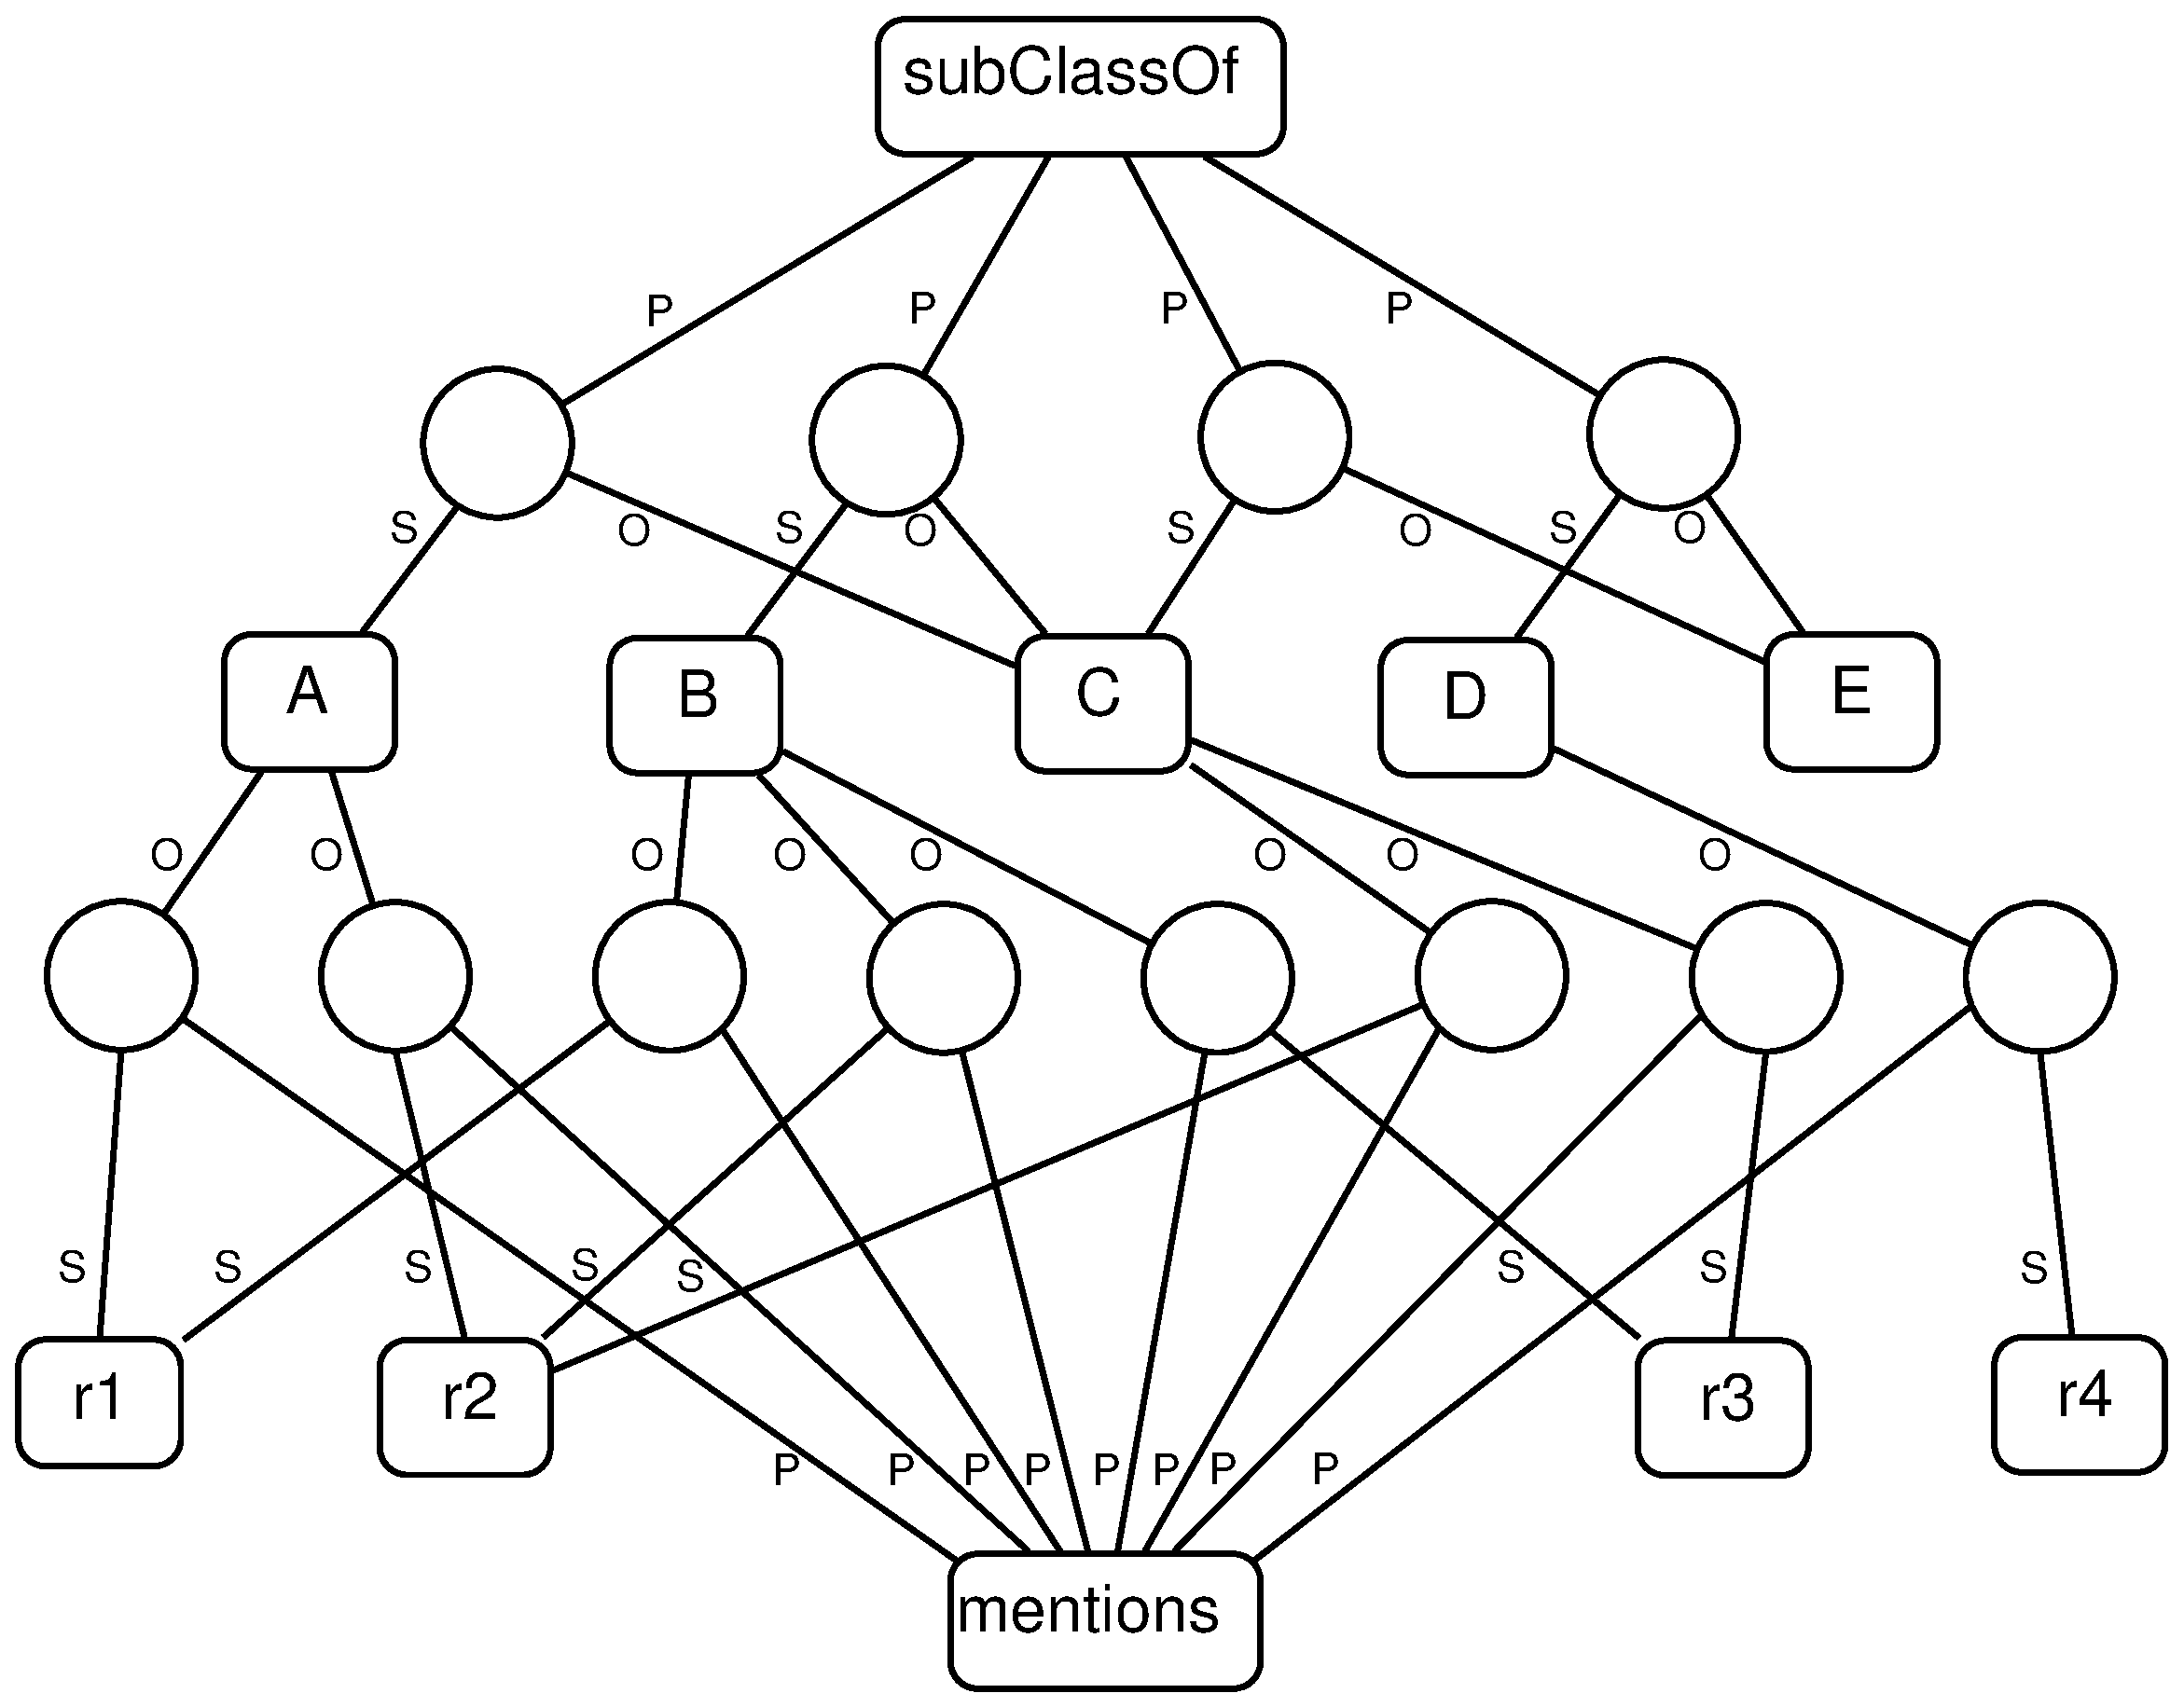
\includegraphics[width=.45\textwidth]{fig/hypergraph_mining.eps}} & \emph{~~~~~~~s \hfill p\hfill o~~~}\\
& $s_1$:~~~\texttt{<A>~~<subClassOf>~~<C>}\\
& $s_2$:~~~\texttt{<B>~~<subClassOf>~~<C>}\\
& $s_3$:~~~\texttt{<C>~~<subClassOf>~~<E>}\\
& $s_4$:~~~\texttt{<D>~~<subClassOf>~~<E>}\\
& \\
& $s_5$:~~~\texttt{<r1>\;~~<mentions>\;~~<A>}\\
& $s_6$:~~~\texttt{<r1>\;~~<mentions>\;~~<B>}\\
& $s_7$:~~~\texttt{<r2>\;~~<mentions>\;~~<A>}\\
& $s_8$:~~~\texttt{<r2>\;~~<mentions>\;~~<B>}\\
& $s_9$:~~~\texttt{<r2>\;~~<mentions>\;~~<C>}\\
& $s_{10}$:~~\texttt{<r3>\;~~<mentions>\;~~<B>}\\
& $s_{11}$:~~\texttt{<r3>\;~~<mentions>\;~~<C>}\\
& $s_{12}$:~~\texttt{<r4>\;~~<mentions>\;~~<D>}\\
& \\
& \\
& \\
& \\
(A) & (B)\\
\end{tabular}
\end{center}
\caption{\label{fig:hypergraph-combined} The RDF bipartite graph representation (A) easily combines both the ontology-annotated data with the ontological relationships (B) based on the information described in Figure~\ref{fig:onto-and-data}.}
\end{figure*}

Formally, the RDF bipartite graph as a unified representation for both data and ontologies is defined as $G=\langle V_v \cup V_s, E \rangle$, where $V_v$ denotes \emph{value nodes} corresponding to components of RDF statements (i.e., subject, predicate, or object), and $V_s$ denotes \emph{statement nodes} corresponding to RDF statements. More specifically, statement nodes can be further divided according to whether they are from data or ontology, i.e., $V_s=V_d \cup V_o$; Value nodes can be divided according to whether they represent rows (records) or columns (attributes) in data, \i.e., $V_d=V_r \cup V_a$. The graph $G$ can be represented in a biadjacency matrix $\mathbf{M}$, where $\mathbf{M}(i,j)$ is non-zero if there is an edge between $\langle V_{v_i}, V_{s_j} \rangle$. For an unweighted graph, the value can be 0/1, and for a weighted graph, any non-negative value. Weights assigned to different paths in the graph are used to distinguish various semantic types or relationships (properties) from the ontology and data, such as class subsumption, ``part\_of", and other general or domain-specific properties.

For example, Figure~\ref{fig:biadjacency-matrices} shows the biadjacency matrices $\mathbf{M}_d$ and $\mathbf{M}_o$ for the RDF bipartite graph shown in Figure~\ref{fig:hypergraph-combined}(A). $\mathbf{M}_d$ and $\mathbf{M}_o$ correspond to the data and ontology part of the RDF bipartite graph respectively. We can see that rows of $\mathbf{M}_d$ and $\mathbf{M}_o$ correspond to \emph{value nodes}, ($V_v$), which can be further divided into row nodes $V_r$ and attribute nodes $V_a$. On the other hand, columns of $\mathbf{M}_d$ are nodes that correspond to RDF statements about data ($V_d$), and columns of $\mathbf{M}_o$ correspond to the ontology ($V_o$). The union of $V_d$ and $V_o$ constitutes the whole set of statement nodes $V_s$ (all circle nodes in Figure~\ref{fig:hypergraph-combined}(A), i.e., $s_1$--$s_{12}$ in Figure~\ref{fig:hypergraph-combined}(B)).

\begin{figure*}[h!t]
\begin{center}
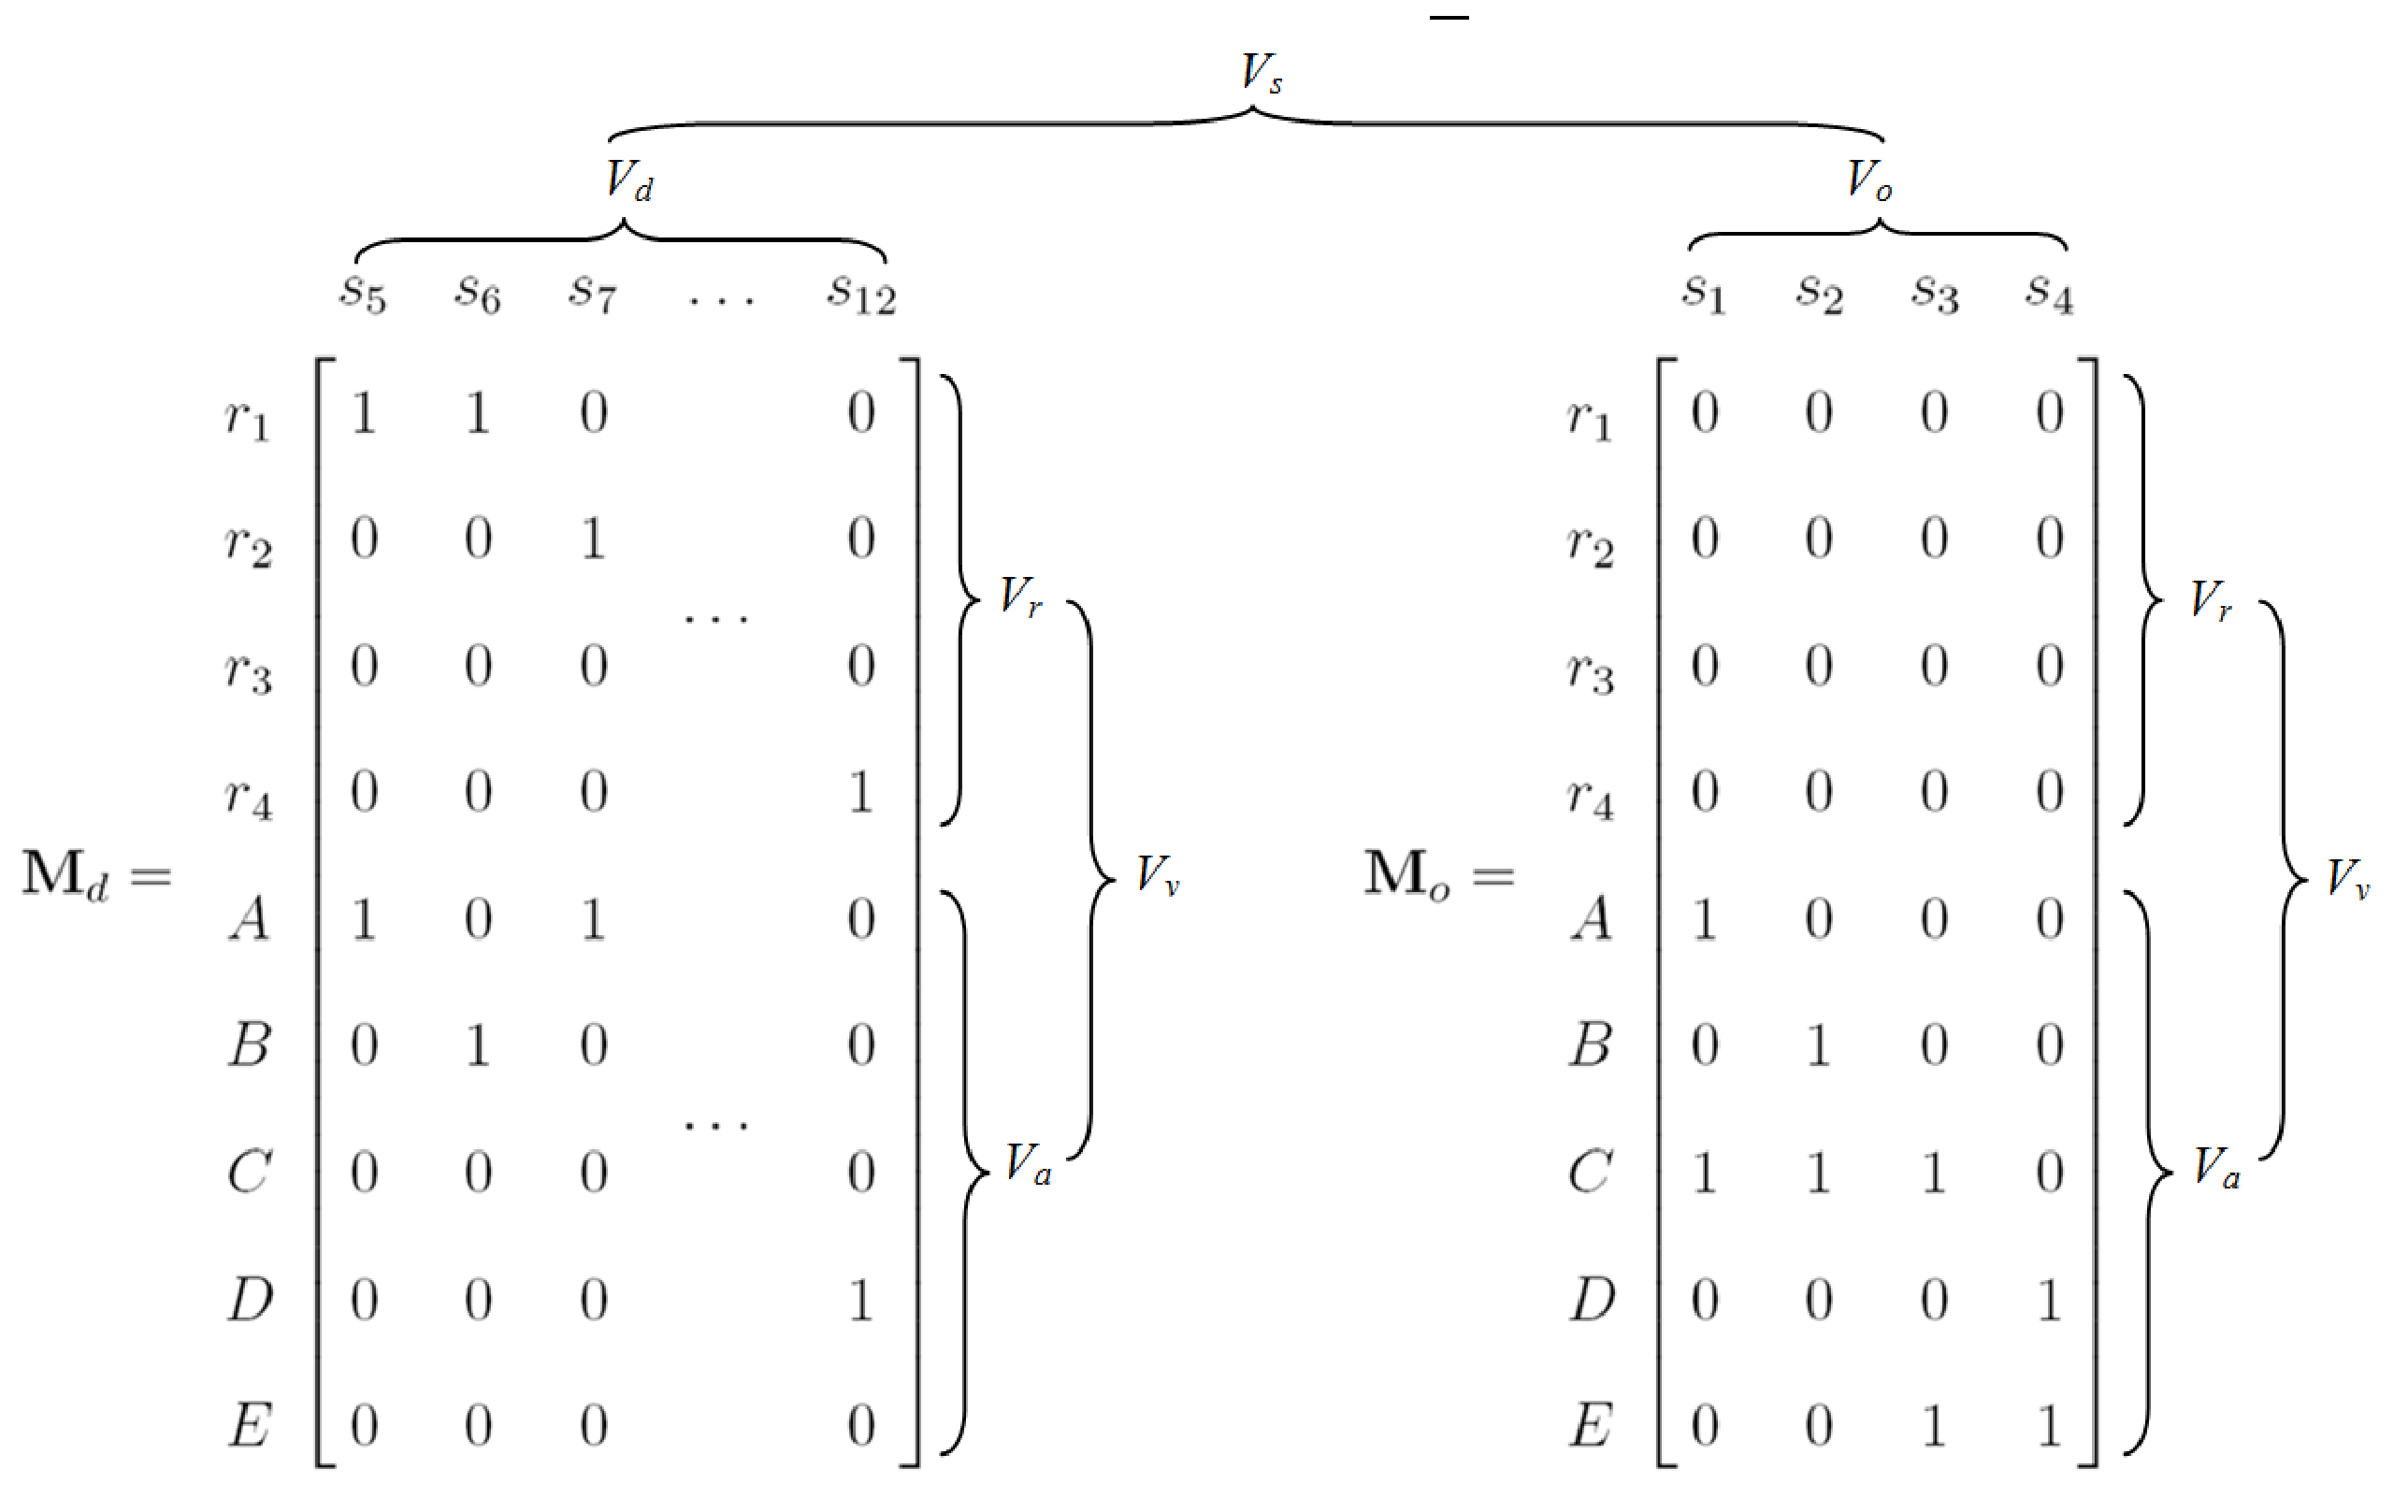
\includegraphics[width=.7\textwidth]{fig/biadjacency-matrices.eps}
\end{center}
\caption[An example RDF bipartite graph and a detailed anatomy of\protect\newline its biadjacency matrix]{\label{fig:biadjacency-matrices} An example RDF bipartite graph and a detailed anatomy of its biadjacency matrix.}
\end{figure*}


From the above example we notice that the biadjacency matrix $\mathbf{M}$ can be split into vertical stripes by statement nodes $V_s$. To obtain the biadjacency matrix $\mathbf{M}$ of the unified RDF bipartite graph in Figure~\ref{fig:biadjacency-matrices}(A), we can simply concatenate $\mathbf{M}_d$ and $\mathbf{M}_o$ horizontally: $\mathbf{M}=\left[\mathbf{M}_d~\mathbf{M}_o\right]$. This gives us a way to construct the matrix modularly from its independent components. In general, if there are $k$ different semantic relationships in ontologies, $\mathbf{M}_o$ can be divided into more vertical stripes $\{\mathbf{M}_{o_i}, i=1\dots k\}$, where $\mathbf{M}_{o_i}$ may represent, for example, the ``part\_of" lattice. Each $\mathbf{M}_{o_i}$ can be distinguished from others by different weights assigned to it. In short, $\mathbf{M}$ is the horizontal concatenation of all weighted vertical stripes as shown in Equation~\ref{eq:horzcat}. The internal block structure of the concatenated biadjacency matrix $\mathbf{M}$ is shown in Equation~\ref{striped_M}.

%horizontal concatenation
\begin{equation}\label{eq:horzcat}
\mathbf{M} = \bigg[w_d\mathbf{M}_d ~~ w_{o_1}\mathbf{M}_{o_1} ~~ w_{o_2}\mathbf{M}_{o_2} ~~ \dots\bigg]
\end{equation}

\begin{equation}
\label{striped_M}
\mathbf{M}=\begin{blockarray}{ccccc}
                ~ & ds & os_1 & os_2 & \dots \\
            \begin{block}{c[c|c|c|c]}
                r   &   \mathbf{M}_{dr}  &   \mathbf{0}   &   \mathbf{0}   &   \dots \\
                \cline{2-5}
                a   &   \mathbf{M}_{da}  &   \mathbf{O}_1 &   \mathbf{O}_2 &   \dots \\
            \end{block}
        \end{blockarray}
\end{equation}


%By developing the unified representation for both data and domain knowledge, and utilizing ontology annotations (\eg,~\cite{LePendu2010}), we can produce a unified RDF bipartite graph, which serves as the basis for mining semantic associations. With additional information from domain knowledge encoded in ontologies, the unified RDF bipartite graph enables us to discover interesting indirect relationships between entities from data. Moreover, the same method also makes it possible to validate relationships between ontological concepts with the help of the present data graph. In the next section, we describe a similarity measure based on random walk with restart on the RDF bipartite graph to capture the semantic association.

With the RDF bipartite graph and its biadjacency matrix defined, in the following, we move on to describe our method to mine semantic associations based on traversing the graph using random walk with restart.


\subsection{Mining Unified RDF Bipartite Graphs}
In this section, we present our method for discovering semantic associations based on the unified RDF bipartite graph of both the ontology and data. Similar to the relevance score~\cite{SunEtal05}, we believe that two items have a strong semantic association if they are related to many similar objects. We denote the similarity score between entities $e_1$ and $e_2$ by $s(e_1, e_2)$, where $s(e_1,e_2) \in [0, 1]$ and $s(e_1, e_2) = 1 \text{ if } e_1 = e_2$. Now the problem of ranking semantic associations in the unified graph can be described as follows.

Given an attribute node $a$ in the unified graph $G = G_d \cup G_o$ and $a \in G_d \cap G_o$ we want to compute a similarity score $s(a, b)$ for all nodes $b(\neq a) \in G_d \cap G_o$. The result is a one-column vector containing all similarity scores with respect to $a$~\cite{Chen_tuplerank:ranking}. We choose to apply random walks with restart (RWR) from the given node $a$, and use the steady-state probability of each other node at convergence as the similarity measure. In other words, the similarity score of node $b$ is defined as the probability of visiting $b$ via a random walk which starts from $a$ and goes back to $a$ with a probability $c$.

In particular, RWR on a bipartite graph works as follows: assume we have a random walker that starts from node $a$. For each step, the walker chooses randomly among the available edges from the current node. After each iteration, with probability $c$, it resets its position back to node $a$. The final steady-state probability that the random walker reaches node $b$ is the similarity score of $b$ with respect to $a$. We choose the random walk approach to compute the relevance score because it gives node $b$ high ranking if $b$ and $a$ are connected by many nodes; this is due to the random walker having more paths to reach $b$ from $a$. The purpose of the periodic restart is to raise the chance that close related nodes are visited more often than other nodes.

The RWR score on bipartite graphs has a desired property that it is easier to compute when the numbers of nodes in the two parts are highly unbalanced. The unified RDF bipartite graph of ontologies and data satisfies this condition because there are generally many more statement nodes than value nodes on large graphs.

In the following, we describe how to algorithmically calculate the RWR-based similarity on the RDF bipartite graph. The algorithm can be used in situations where, for example, users are interested in knowing products that are usually bought together in the same transactions by different customers, or common side effects of the same drugs prescribed to different patients, etc.

Given a biadjacency matrix $\mathbf{M}$ in Equation~\ref{eq:horzcat} for the unified RDF bipartite graph $G$, we can construct the adjacency matrix $\mathbf{A}$ of $G$ as following:
\[
\mathbf{A}=\left[
               \begin{array}{cc}
                 \mathbf{0}   & \mathbf{M} \\
                 \mathbf{M}^T & \mathbf{0} \\
               \end{array}
             \right].
\]
The probability of a random walker taking a particular edge $\langle a,b\rangle$ from a node $a$ while traversing the graph is proportional to the edge weight over the total weight of all outgoing edges from $a$, i.e., $\mathbf{P}(a,b)=\mathbf{A}(a,b)/\Sigma_{i=1}^{m+n}\mathbf{A}(a,i)$. Therefore, the Markov transition matrix $\mathbf{P}$ of $G$ is constructed as: $\mathbf{P}=normc(\mathbf{A})$, where $normc(\mathbf{A})$ normalizes $\mathbf{A}$ such that every column sum up to 1.

Given the transition matrix $\mathbf{P}$, we can calculate the similarity scores using the following steps. First, we transform the input attribute node $a$ into a $(k+n) \times 1$ query vector $\mathbf{q}_a$ with 1 in the $a$-th row and 0 otherwise. Second, we need to compute a $(k+n)\times 1$ steady-state probability vector $\mathbf{u}_a$ over all nodes in $G$. Last we extract only the steady-state probabilities of row nodes in $\mathbf{M}$ (corresponding to value nodes in the RDF bipartite graph) as the output similarity score vector. Notice that $\mathbf{u}_a$ can be computed by an iterated method from the following iterative equation.

Let $c$ be the probability of restarting random-walk from the node $a$. Then the steady-state probability vector $\mathbf{u}_a$ satisfies
\begin{equation}
\label{eq:steady-state}
\mathbf{u}_a=(1-c)\mathbf{P}_A\mathbf{u}_a+c\mathbf{q}_a~.
\end{equation}

\renewcommand{\algorithmicrequire}{\textbf{Input:}}
\renewcommand{\algorithmicensure}{\textbf{Output:}}
\begin{algorithm}
\caption{Calculate Semantic Association}
\label{alg1}
\begin{algorithmic}
\REQUIRE query attribute $a$, bipartite matrix $M$, restarting probability $c$, tolerant threshold $\epsilon$
\ENSURE similarity vector $\mathbf{u}_a(1:k)$
\STATE $\mathbf{q}_a \Leftarrow \mathbf{0}$
\STATE $\mathbf{q}_a(a)=1$ (set $a$-th element of $\mathbf{q}_a$ to 1)
\WHILE{$|\Delta\mathbf{u}_a| > \epsilon$}
\STATE \[
    \mathbf{u}_a = (1-c)  \left[ \begin{array}{c}
        normc(\mathbf{M})\mathbf{u}_a(k+1:k+n);\\
        normc(\mathbf{M}^T)\mathbf{u}_a(1:k)
    \end{array} \right] + c\mathbf{q}_a
\]
\ENDWHILE
\RETURN $\mathbf{u}_a(1:k)$
\end{algorithmic}
\end{algorithm}

The iterative update of $\mathbf{u}_a$ can be performed as shown in Algorithm~\ref{alg1}. The while loop is modified from Equation~\ref{eq:steady-state} to avoid materializing $\mathbf{A}$ and $\mathbf{P}$ for scalability. 